\clearpage
\setcounter{page}{1}
\maketitlesupplementary



\section{Computing the Upper Confidence Bound Score of a Game State}
\label{sec:ucb_score}
% Store the equation in the appendix.
The $UCB$ score is an intuitive equation, it promotes exploration and exploitation. It's derived based on following four relations:
\begin{enumerate}
  \item Higher prior $p$ (given by the policy) should \emph{raise} the score
  \item Higher number of times the node's parent has been visited $n_{parent}$, should \emph{raise} the score.
  \item Higher number of times this node has been visited, $n$, should \emph{lower} the score
  \item Higher ratio of value per visits, $V$, of this node, should \emph{lower} the score
\end{enumerate}
\begin{align}
  UCB &= V + P \\
  V &= \begin{cases}
    -\sum_{v\in children} \frac{v}{n} &\quad \text{if} \, n > 0 \\
    0 &\quad \text{otherwise}
  \end{cases} \\
  P &= \frac{p\sqrt{n_{parent}}}{n + 1}
\end{align}

\section{Pseudocode for the Monte Carlo Tree Search}
\label{sec:mcts_code}

\begin{algorithm}[h]
  \caption{Monte Carlo Tree Search (MCTS)}
  \label{alg:mcts}
  \begin{algorithmic}[1]
  \Function{run\_simulations}{$n_{sims}$}
  \State Initialize root node with the current game state.
  \For{$n_{sims}$}
      \State current\_node $\gets$ root
      \State Intialize search\_path to empty list
      \While{current\_node isn't expanded}
          \State Select the next node based on $UCB$
          \State Add the selected node to the search\_path
      \EndWhile
      \If{the game ends at the current node}
          \State value $\gets 1$ if model wins, $-1$ otherwise
      \Else
          \State Expand the current node and predict value
      \EndIf
      \State Add the value to nodes along the search path.
  \EndFor
  \State Compute probabilities for each action based on visit counts.
  \State Select the action with the highest visit count as the best move.
  \State \Return the best action and its probabilities.
  \EndFunction
  \end{algorithmic}
  \end{algorithm}

\section{Loss Plot}
\label{sec:loss_plot}
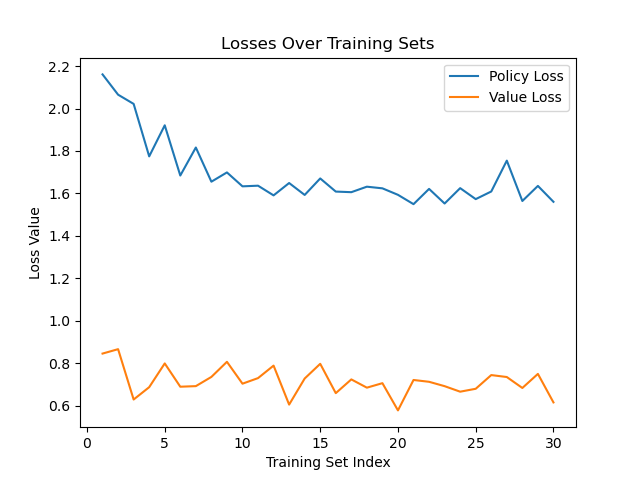
\includegraphics[width=\linewidth]{plots/correct_loss.png}

\section{Pseudocode for the Minimax Algorithm}
\label{sec:minimax_code}
\begin{algorithm}[h]
  \caption{Minimax Algorithm for Tic-Tac-Toe}
  \begin{algorithmic}[1]
  
  \Function{Score}{board, $depth$}
      \If{PlayerWins(board)}
          \State \Return $10 - depth$
      \ElsIf{OpponentWins(board)}
          \State\Return $-10 + depth$
      \Else
          \State\Return 0
      \EndIf
  \EndFunction

  \Function{Minimax}{board, depth, isPlayer}
      \If{GameOver(board)}
          \State\Return{Score(board, depth)}
      \EndIf
      
      \State{moves} $\gets$ GetValidMoves(board)
      
      % \For{each move in moves}
      %     \State{newBoard} $\gets$ MakeMove(board, move)
      %     \State{score} $\gets$ Minimax(newBoard, depth + 1, $\neg$isPlayer)
          
      %     \If{isMaximizer}
      %         \If{score > bestScore}
      %             \State{bestScore} $\gets$ score
      %             \State{bestMove} $\gets$ move
      %         \EndIf
      %     \Else
      %         \If{score < bestScore}
      %             \State{bestScore} $\gets$ score
      %             \State{bestMove} $\gets$ move
      %         \EndIf
      %     \EndIf
      % \EndFor
      \State Initialize scores as a list
      \For{each move in moves}
        \State Initialize newBoard with move
        \State scores $\gets$ Minimax(newBoard, depth+1 $\neg$ isPlayer)
      \EndFor
      \If{isPlayer}
        \State \Return move and score that maximizes score
      \Else
        \State \Return move and score that minimizes score
      \EndIf
  \EndFunction
  
  \end{algorithmic}
  \end{algorithm}

% \section{Policy and Value Network Diagrams}
% 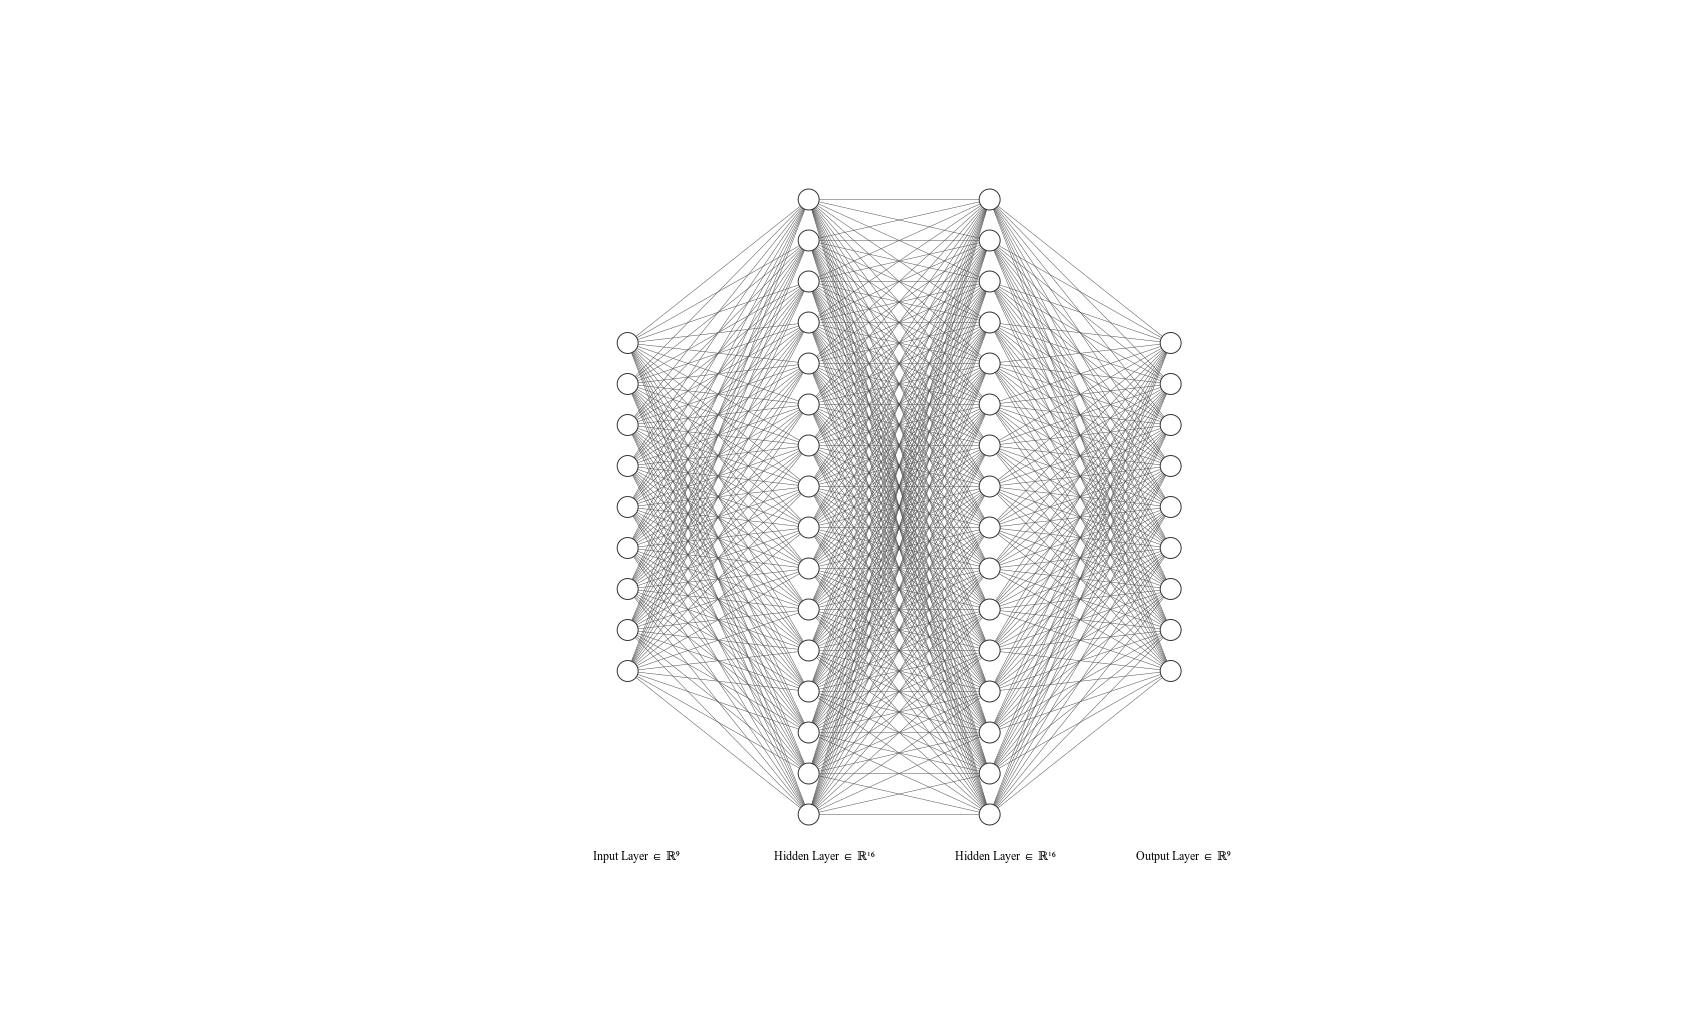
\includegraphics[width=\linewidth]{plots/policy.png}
% 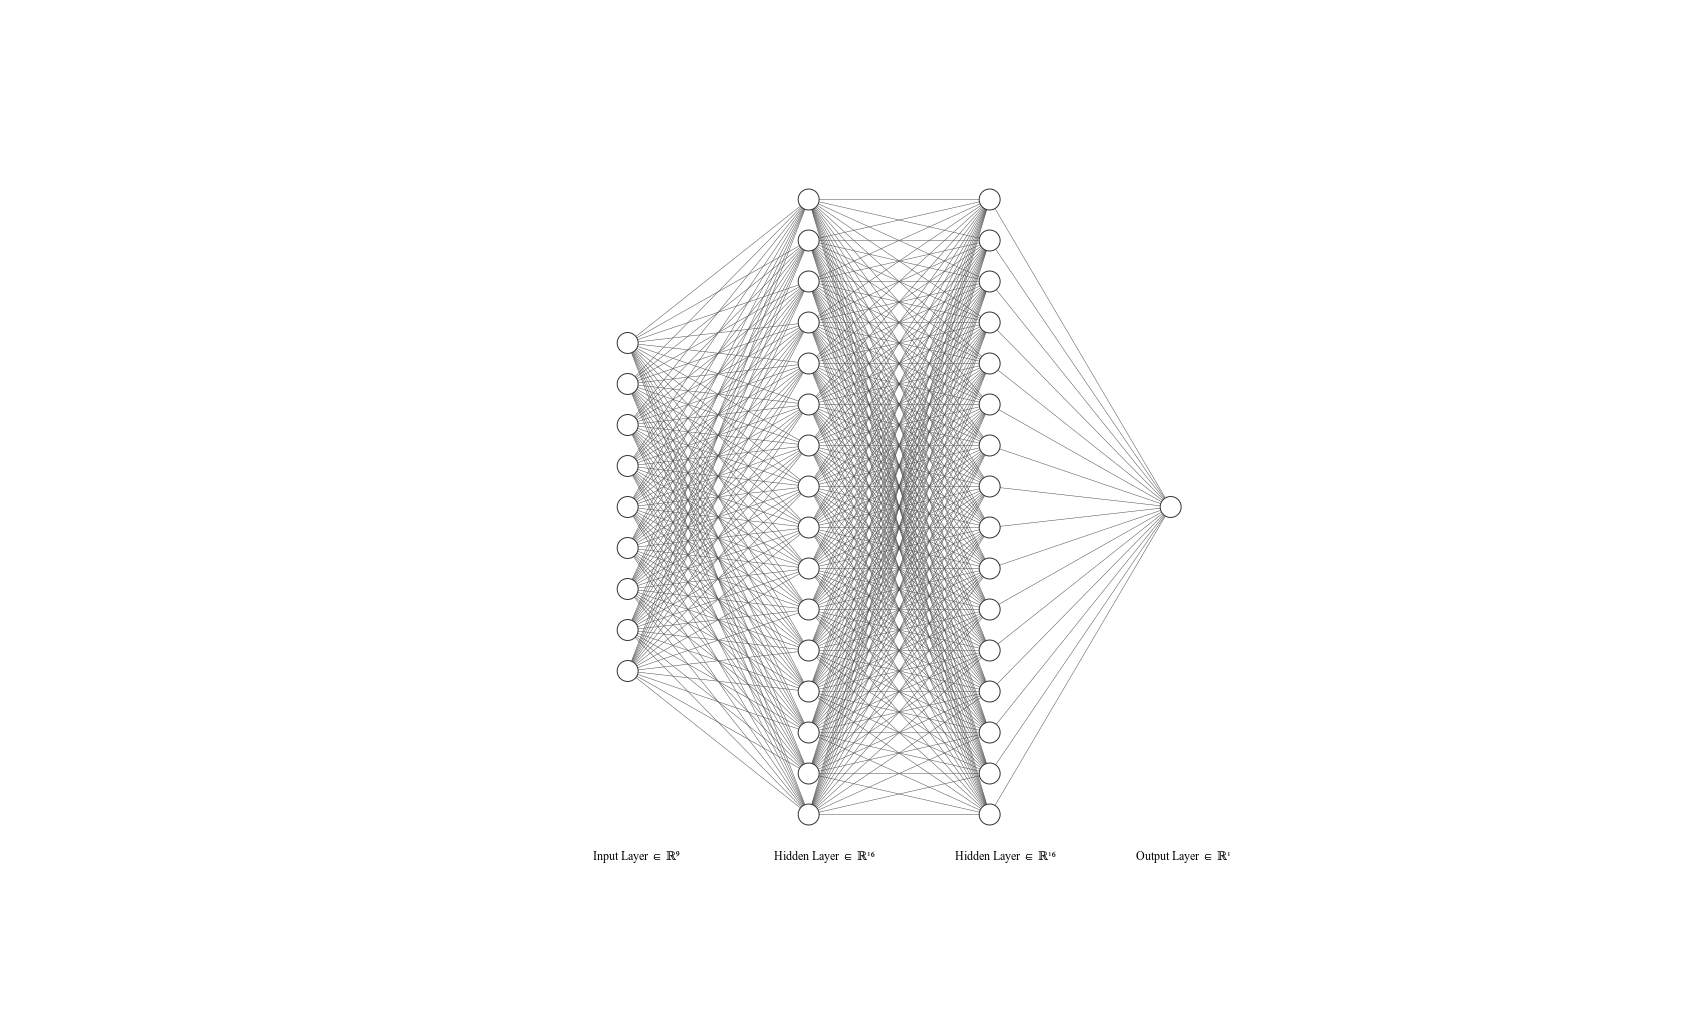
\includegraphics[width=\linewidth]{plots/value.png}